
\chapter{Installation}
\label{txt:installation}
Tellervo is made up of two packages; the Tellervo desktop application and the Tellervo database server.  Tellervo was designed primarily for laboratories with multiple users, each running the Tellervo desktop application on their own computer connecting to a single central server containing the lab's data.  In this situation the Tellervo server would be run on a separate computer to those running the desktop client, but this need not necessarily be the case.  It is perfectly possible to run both the server and the client on the same computer.  This is likely to be the situation if you simply want to try out Tellervo, if you don't have a separate server, or if you do not work in a multi-user laboratory.

Tellervo can be run without access to a Tellervo server, however, in offline mode (known as Tellervo-lite) it has a greatly reduced functionality.  Without access to a database the mapping, barcoding, metadata support, permissions handling etc are all disabled.  Tellervo-lite functions as a basic data collection tool saving to a variety of legacy file formats.  While this may be adequate for casual dendro users, we urge you to install the Tellervo server too and make full use of the functionality that it provides.


\section{Server installation}
\index{Installation!Server}
To make full use of the potential of the Tellervo desktop application you will require access to a Tellervo server.  If you are running Tellervo in a lab where the Tellervo server has already been set up by your systems administrator, you can skip this section.

The Tellervo server is made up of a number of components, which unlike the desktop client, can't be easily combined together into cross-platform packages.  Although all the constituent components are open-source and available for all major platforms, building and maintaining separate packages for each platform is too large a task for a small development team.  To conserve resources, we therefore made the decision to utilize Virtual Machine technology to ensure that the Tellervo server could still be run on all major operating systems.  This means that we can package the Tellervo server for a single operating system (Ubuntu Linux) and then distribute it as a Virtual Appliance that can be run as a program on your normal operating system. 

The Tellervo server is therefore available via three methods.  The first is as a VirtualBox\footnote{Note that the Tellervo appliance is provided in the open standard format OVA.  You should be able to run the appliance in other Virtual Machine applications (e.g. VMWare, Citrix etc) but the OVA standard is very young and changing fast.  We recommend sticking with VirtualBox until the standard stabilizes. } Virtual Appliance which can be run on any major operating system and we strongly recommend that you stick with this option unless you are experienced with Linux and running servers.  The second option is to intall the native Ubuntu package on an Ubuntu Linux server. The source code for the server is also available so it is perfectly possible for more experienced users to set up the Tellervo server to run natively on other platforms.  But to do this you will require a good knowledge of Apache 2, PHP and PostgreSQL.  Choose the most applicable method and follow the instructions in the following sections.


\subsection[Install as Virtual Appliance]{Install as Virtual Appliance (recommended method)}
\label{txt:virtualAppliance}
\index{Virtual appliance}
To run the Tellervo server Virtual Appliance, you will first need to download and install VirtualBox from \url{http://www.virtualbox.org}.  Installation packages are available for Windows, MacOSX, OpenSolaris and many Linux distributions.

Once you have VirtualBox installed, you will then need to download the Tellervo server from the Tellervo website \url{http://www.tellervo.org/download}.  This package contains a bare-bones Ubuntu Linux server with everything required to run the Tellervo server installed and ready to use.  As VirtualBox, the entire Ubuntu operating system and Tellervo server components are all open source there are no license fees to pay.

\begin{wrapfigure}{r}{0.5\textwidth}
  \begin{center}
    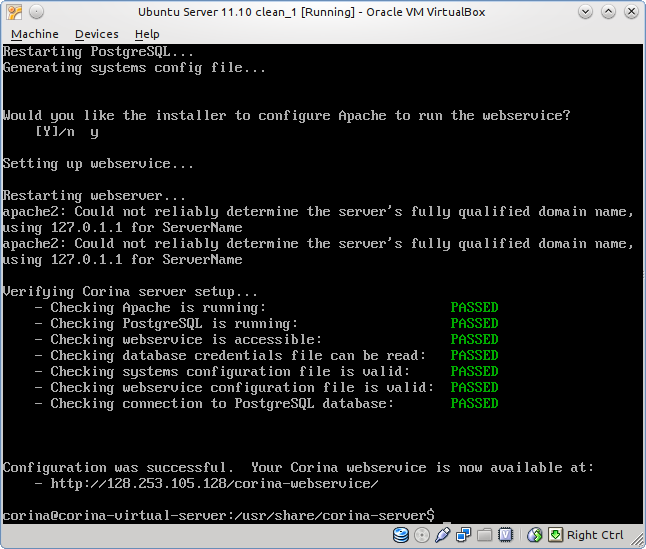
\includegraphics[width=0.48\textwidth]{Images/serverconfig.png}
  \end{center}
  \caption{Screenshot of VirtualBox running the Tellervo server.  The console contains the results of the tests run at the end of the configuration routine.}
  \label{fig:serverconfig}
\end{wrapfigure}

\begin{enumerate}
 \item Open VirtualBox and go to \menutwo{File}{Import Appliance}
 \item Press the choose button and locate the virtual appliance file that you downloaded from the website\footnote{If you are using an older version of VirtualBox it may expect an OVF rather than the OVA file provided.  The OVA file is a tar file containing several files required by VirtualBox including an OVF file.  If you rename the extension of the OVA file to tar then extract the contents to a folder using a tools like WinRAR you should then be able to continue.}
 \item Rename the server if you choose, then press the finish/import button
 \item Once the server is installed, highlight it in the virtual machine list and press the `settings' button
 \item Go to `Network' and choose `Attached to Bridged Adapter'.  You may also like to give the system more RAM if you have powerful machine
 \item Click ok, then back on the main page, press the `run' button
 \item Read and accept the information about how to gain and release control of the keyboard in VirtualBox
 \item The server will boot and eventually present you with a command line login screen.  Log in with the following temporary details:
    \begin{description}
      \item[Username] : tellervo
      \item[Password] : dendrochronology
    \end{description}
 \item Once you are logged in the server will automatically ask you a series of questions 
 \item Answer the questions and the configuration will finish by testing your new server (see figure \ref{fig:serverconfig}). 
 \item Note down the URL of your new Tellervo webservice as you will need to enter this when you start your Tellervo desktop client.  If you need to know the URL at a later date you can run the tests again by typing: \code{tellervo-server --test}
 \item You can now install and run the Tellervo Desktop application (see section \ref{txt:desktopinstall})
\end{enumerate}

To save on download size and disk space only the essential packages to make the server run have been installed.  This means there is no graphical interface just a command line.  Hopefully this should not be a problem as once set up, the only interaction needed with the Virtual Appliance will be through the normal Tellervo desktop application.  If you would prefer to use a graphical interface to the server this can be easily installed.  See chapter \ref{txt:servermaintenance} for further details.

There are a number of limitations caused by distributing the server software in this way. The operating system has already been configured to use networking without a proxy server, so if your computer requires a proxy then you won't be able to connect to the Internet.  Please contact the developers for more details.

VirtualBox has a number of methods for providing network connectivity to the Tellervo virtual appliance.  The default setup described above is to use \textbf{bridged networking}.  This makes the virtual server appear as if it was another physical computer on your network with its own IP address.  This works best in most situations, but can cause problems if your network administration is particularly strict.  It is also not suited to those installing Tellervo Server on a laptop which is used on different networks, especially via wifi.  If you have problems with bridged networking, then it may be better to use one of the alternatives listed below.

The first network alternative is to use \textbf{host-only networking}.  To use this you simple select your server in VirtualBox, click settings then on the network tab choose host-only adapter.  This setting means that your server will only be visible to the physical computer you are running Tellervo server on.  This may not be a problem (it may even be desirable) if you are installing for your personal use but of course it is not suitable if you are intending to share the server with colleagues.

The second network alternative is to use \textbf{NAT networking}.  NAT stands for Network Address Translation and means that requests and responses sent to/from your physical computer are intercepted and forwarded on to the virtual Tellervo server.  Instead of Tellervo server having its own IP address, Tellervo clients wanting to talk to the server send requests to your physical computer.  This has the benefit of being more likely to work if your institution has strict network policies.  The main drawback is that it takes a little more effort, and perhaps requires a better understanding of systems administration to set up.  

With your virtual machine powered off, select it in VirtualBox, click settings and go to the network tab.  Change the network type to NAT and then click the port forwarding button.  Add an entry to the list:
\begin{description}
 \item[Name] - TellervoHTTP
 \item[Protocol] - TCP
 \item[Host Port] - 8080
 \item[Guest Port] - 80 
\end{description}
You can leave the other fields blank.  The host port is the port that your Tellervo users connect to.  The normal port that users connect to for web services is port 80, however, on most secure operating systems (e.g. Linux and OSX) you cannot port forward to ports below 1024, although it should be possible in Windows.  If you are running Windows you may therefore be able to use a host port of 80.  If you use 8080 (or any other port other than 80) you will need to include this in the URL of your webservice when you try to connect.  The other complication of using NAT networking is that the URL provided by the Tellervo server configuration utility is incorrect as the server has no way of knowing that NAT is being used.  The URL that you need to use to connect to is: \url{http://ip.of.your.physical.machine:8080/tellervo/}  


\subsection{Ubuntu native installation}
\label{txt:installnativeserver}
If you are fortunate enough to be running Ubuntu then the native Ubuntu deb package is the best and easiest method for installing the Tellervo server, otherwise see section \ref{txt:virtualAppliance} to install the server as a Virtual Appliance.  

To install the Tellervo server in Ubuntu simply download the deb package from the Tellervo server \url{http://www.tellervo.org/download} and install with your favourite package manager.  For instance, to install from the command line simply type: \code{sudo dpkg --install tellervo-server.deb}.  If you haven't got all the required dependencies already installed dpkg will return an error.  This can be fixed by running \code{sudo apt-get install -f} which will install all the missing packages, and will automatically allow dpkg to run to completion.  

The package will automatically run a configuration script to assist with creating a database user, building the Tellervo PostgreSQL database, setting database permissions and setting up the Apache webservice.  The configuration ends with a test routine to check all services are set up correctly and if so, will provide you with the URL of the newly configured Tellervo webservice.

\subsection{Advanced install on other operating systems}
\label{txt:installadvancedserver}
As mentioned previously, the limited resources available for Tellervo development means that we have been unable to produce native installers for platforms other that Ubuntu.  The VirtualBox method can be used on all modern operating systems so we strongly suggest you stick with this method.  However, if you are an experience systems administrator and are feeling brave, it is possible to set up the Tellervo server manually.  

\index{Dependencies!Server}
The Tellervo server is essentially a PostgreSQL database accessed via a PHP webservice running on Apache 2.  The following dependencies are therefore required: postgresql-9.1; postgis; postgresql-contrib-9.1; postgresql-9.1-pljava; sun-java6-jre; apache2; php5; php5-pgsql; php5-curl; php5-mhash.

The basic procedure for installation is as follows:

\begin{itemize*}
 \item Install all dependencies
 \item Create PostgreSQL database from Tellervo template SQL file
 \item Set up a database user and provide access to the server in the pg\_hba.conf file
 \item Give this user read and write permissions to the database
 \item Copy the webservice code into a web accessible folder
 \item Set up Apache to see this folder by creating an entry in the sites-enabled folder
 \item Restart PostgreSQL and Apache and check you can access the webservice from a web browser
\end{itemize*}




\section{Installing the desktop application}
\label{txt:desktopinstall}
\index{Installation!Desktop application}
Installation packages for the Tellervo desktop application are available for Windows, MacOSX and Ubuntu Linux.  Tellervo can also be run on other operating systems as long as they support Java 6 or later\footnote{Tellervo was initially developed against Sun Java 6 JRE, however, now OpenJDK6 is routinely used.  See section \ref{txt:java}, page \pageref{txt:java} for more information.}.

To install Tellervo, download the installation file for your operating system from \url{http://www.tellervo.org/download}. The website should provide you with a link to the installer for your current operating system:

\begin{description}
\item 
\includegraphics[width=3mm]{Images/windows.png} \textbf{Windows} -- Run the setup.exe and follow the instructions. If you do not have Java installed the installer will direct you to the Java website where you can get the latest version. Once installed, Tellervo can be launched via the Start menu.  Please note that Windows (and possibly also your anti-virus software) may warn you that the installation program is not commonly downloaded and may be dangerous.  You will see that the installation package is digitally signed by the University of Arizona indicating that the file has not been tampered with.  As long as you trust the Tellervo developers you can safely install the program.

\item 
\includegraphics[width=3mm]{Images/mac.png} \textbf{Mac OS X} -- As mentioned above, Tellervo requires Java 6. Although MacOSX ships with Java installed, unfortunately Apple have been very slow to provide Java 6. Although it was released in 2006, it was not until August 2009 that Apple made Java 6 available as part of v10.6 (Snow Leopard). Tellervo can therefore only be run on Snow Leopard or later\footnote{The Snow Leopard requirement for Mac computers means that Tellervo cannot be run on older PowerPC-based MacOSX computers.  However, if you have old PowerPC iMacs you could consider replacing the operating system with a modern Linux distribution like Ubuntu.  Linux continues to support PowerPC architecture even in the most recent releases.  You will of course not be able to run any of your other exisiting MacOSX software.}. To install Tellervo, download then open the zip file and drag the Tellervo.app into your applications folder.  To use the 3D mapping or measuring platform hardware in Tellervo you will also need to install the `Tellervo Drivers' package.  Note that users of OSX 10.8 (Mountain Lion) and later may be told that the package is broken.  This is due to Apple's new GateKeeper tool which by default won't allow non-Apple unsigned applications to run.  See section \ref{txt:malware} for more information.   

\item 
\includegraphics[width=3mm]{Images/ubuntu.png} \textbf{Ubuntu Linux} --  A deb file is available which was designed for use on Ubuntu distributions but should work on any Debian based system. Install using your favorite package management system or from the command line like this: e.g. \code{sudo dpkg --install tellervo.xx.xx\_all.deb} On Ubuntu and similar distributions, the package should add a Tellervo shortcut to your applications menu. Alternatively you can start Tellervo from the command line by typing tellervo.  For other Linux distributions you are probably better off using the standard Java executable described below.  Note though that you will need to manually install serial port and 3D graphics libraries to use these features in Tellervo.  If there is demand for a package for other Linux distributions we may make these available in the future.  For instance, basic RPMs have been produced but we do not have the time or resources to test these at the moment.

\item 
\includegraphics[width=3mm]{Images/java.png} \textbf{Other operating systems} -- Make sure you have Java 6 installed, then download the Tellervo jar file to your hard disk. You can run Tellervo from the command line by typing: \code{java -jar tellervo.jar}  Note that several native libraries are required to enable Java to interface with your serial port and 3D graphics hardware.  If you want to take advantage of these features in Tellervo you will need to manually install these libraries.  Please contact the Tellervo developers for more information.
\end{description}

Once you have installed your Tellervo Desktop application and you have access to a Tellervo server you are now ready to launch Tellervo for the first time.


\subsection{Malware and broken package warnings}
\label{txt:malware}

The MacOSX package for Tellervo is currently `unsigned'.  By default any application run on MacOSX Mountain Lion (10.8) and later must be signed with an Apple certificate to run.  Rather frustratingly rather than explain this OSX simply reports that the package is `damaged'.

The cleanest method for fixing this is for us (the developers) to pay a certificate from Apple.  However, with tight budgets all around, justifying spending hundreds of dollars each year just to digitally sign the installation packages is very difficult.  Until we find the funds to do this sustainably, you will need to change some security settings.  First, go to \menutwo{System Properties}{Security and Privacy}.  By default it is set to allow applications from `Apple and known developers'.  You will need to change this to `any developer' to be able to run Tellervo. With this set, when you run Tellervo you will be warned that the package is untrusted but it will then allow you to proceed.


\subsection{First time launch}
\index{Wizard, Setup}
When you launch Tellervo for the first time you will be presented with a setup wizard (figure \ref{fig:setupwizard}).  Following the wizard to configure the main settings required before you can begin to use Tellervo.  If you want to re-run this wizard at any time you can do so from the entry in the Help menu. You can also manually edit all these settings from the Tellervo preferences dialog which can be found in \menutwo{Edit}{Preferences}.

\begin{figure}[hbtp]
  \centering
    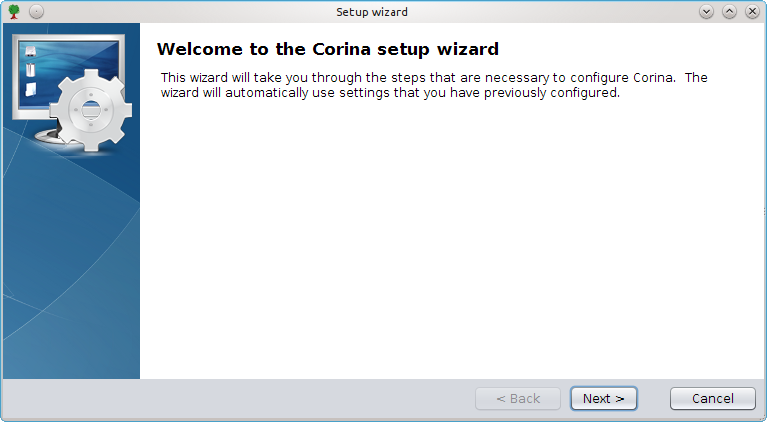
\includegraphics[width=0.6\textwidth]{Images/setupwizard.png}
  \caption{The Tellervo setup wizard will launch the first time you start Tellervo.}
  \label{fig:setupwizard}
\end{figure}

The pages of the wizard include:

\begin{description}
 \item[Network connection] -- this configures how your computer accesses the internet.  Most users will be able to use the default `Use system default proxy settings' option here, but if you know that your computer is behind a corporate proxy server you may choose to manually provide the settings.
 \item[Configuring the Tellervo server] -- Tellervo comes in two parts: the Tellervo desktop client that you are using; and the Tellervo server which runs the database that stores your data.  If you are working in a lab your systems administrator may have already set up the Tellervo server and given you the URL to connect to.  Alternatively, you may have already installed the Tellervo server yourself.  If so the installation program should have given you the URL. If you don't want to take advantage of the full capabilities of Tellervo you can opt to disable database integration.  If you do not configure a Tellervo server you will be left with a basic file-based dendro data collection tool.
 \item[Measuring platform configuration] -- the next page enables you to configure measuring platform hardware attached to your computer.  Some measuring platforms have fixed settings in which case the port settings will be set automatically, but others can be changed in the hardware and must be set explicitly here. Use the `Test Connection' button to make sure that Tellervo can successfully communicate with your platform.
 \item[Tutorial videos] -- Once you've completed the wizard you will be given the option of viewing tutorial videos explaining how to use Tellervo.  You can access these at any time via the Help menu or through the Tellervo website.
\end{description}


Assuming that you have configured a Tellervo server, once you have finished the wizard you will be presented with a login dialog (figure \ref{fig:login}).

The username and password details requested are your Tellervo login credentials (not your system or network credentials) provided to you by your systems administrator.  If you are using your own Virtual Appliance server, the default admin user details are provided in section \ref{txt:passwords}, page \pageref{txt:passwords}.  The dialog gives you the option for saving your username and/or password if you prefer.  We recommend using this feature only on personal machines.  You may choose to cancel the login if you like and Tellervo will continue to load, however, you will not have access to the Tellervo database therefore very few functions will be available to you.

\begin{wrapfigure}{r}{0.5\textwidth}
  \begin{center}
    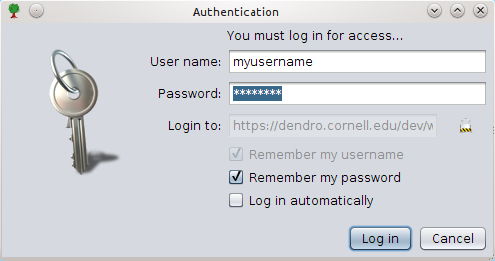
\includegraphics[width=0.48\textwidth]{Images/login.png}
  \end{center}
  \caption{Tellervo server login dialog.}
  \label{fig:login}
\end{wrapfigure}

Once you have logged in you will be presented with the Tellervo home screen.  This contains the main menus for the program as well as quick-link icons for creating new records, opening existing records and importing existing data files to the database.


\subsection{Mapping support}
\index{Mapping}
Tellervo includes 3D mapping for visualization of sampling locations. Although this is not necessary for most tasks, to make use of the mapping functions you will require a OpenGL 3D capable graphics card. To check whether your computer already supports 3D mapping, open Tellervo, go to Admin, then Site map.  Tellervo will warn you if your graphics card is not supported.

All MacOSX computers should automatically support OpenGL.  Most Windows and Linux computers made since 2006 should also support OpenGL, however, this does require proper drivers to be installed. In some cases Windows computers may include a compatible graphics card, but may only have the default Windows video drivers installed.  If you are having trouble with the mapping in Tellervo make sure you have installed the most recent drivers for your graphics card.  Linux users may be required to install proprietary graphics drivers.  

The mapping component of Tellervo makes use of NASA's open source World Wind Java.  NASA's website \url{http://worldwind.arc.nasa.gov/} contains further information and instructions that you may find helpful if you are having problems getting the mapping to work.  


\section{Upgrading Tellervo desktop}

There are no special requirements for upgrading the Tellervo desktop client.  You need simply install the new version over the top of your previous version.  Any personal settings will be maintained after the upgrade.


\section{Upgrading Tellervo Server}

The process for upgrading your server is the same regardless of whether it is running in a VirtualBox virtual machine or on a native Linux server.  As with any upgrade, the first thing you need to do is backup your data (see section \ref{txt:BackupVA}, page \pageref{txt:BackupVA}).  We cannot be held responsible for loss of data in the event something goes wrong during the upgrade process.  

Open your Tellervo server and log in to the command line.  Then type the following commands:

\code{cd /tmp}
\code{wget http://www.tellervo.org/url-of-the-updated-package.deb}
\code{sudo dpkg --install tellervo.x.x.x.deb}

The first line changes your current directory to the temporary folder.  The second command downloads the new package from the Tellervo server.  Make sure you enter the correct URL to the package you are upgrading to.  The final command installs the new package.  Again make sure you have the correct file name specified here. If all goes well, your webservice and database will be upgraded to the latest version and the server test routine will run to confirm all is correct.  If the server gives you any errors or warnings, please contact the developers for further assistance.

\section{Uninstalling}

We understand that Tellervo will never suit the requirements of all users, but as an open source product, we would really appreciate feedback as to why it didn't work for you.  Without this feedback it is difficult to prioritize future development.

\subsection{Tellervo desktop application}
For Windows users, Tellervo desktop can be uninstalled using the standard add/remove programs feature in control panel, or via the item in the Tellervo start menu.  Mac users should simply delete the application from their applications folder.  Linux users should use their prefered package management tool e.g.\ from the command line:
\code{sudo dpkg --remove tellervo}

\subsection{Tellervo server}

\warn{Please note that uninstalling the Tellervo server will delete your Tellervo database and all the data it contains.  Make sure that you export any data you need before doing uninstalling.}

If you are running the Tellervo server as a virtual appliance simply follow the uninstall instructions for VirtualBox.  If you are running Tellervo server as a native Linux server, you should use your preferred package mangement tool e.g.\ from the command line:
\code{sudo dpkg --remove tellervo-server}







